% #############################################################################
% This is Chapter 1
% !TEX root = ../main.tex
% #############################################################################
% Change the Name of the Chapter i the following line
\fancychapter{Introduction}
\cleardoublepage
% The following line allows to ref this chapter
\label{chap:intro}

In recent years, urban air pollution has been a growing worry among countries and their citizens mainly due to its negative impact on population health and life quality. It is a global challenge for governments, which make big investments to decrease air pollution, to raise the awareness of their citizens and to implement effective policies and interventions to tackle the problem. By monitoring and forecasting air quality it is possible to have a better understanding on its evolution and on how to proceed to improve it \cite{WHO2018}.

% #############################################################################
\section{Topic Overview}

Currently, air pollution is a major environmental problem, as it is estimated by the \ac{WHO} that 9 out of 10 people breathe air containing high levels of pollutants and that every year there are 7 million deaths caused by outdoor and indoor air pollution. Outdoor air pollution caused approximately 4.2 million deaths in 2016 and is currently estimated to be responsible for 25\% of adult deaths from strokes, 43\% from chronic obstructive pulmonary disease and 29\% from lung cancer \cite{WHO2018}. WHO states that it affects children neural and motor development and damages their lung function, even at lower levels of exposure. This is a worrying situation since globally, 93\% of the world’s children under 15 years are exposed to \ac{PM2.5} above the WHO guidelines \cite{WHO2018a}.

Air pollution also has a negative impact on society in other ways, such as by stunting plant growth, lowering agricultural productivity and by reducing city progress and attractiveness to citizens, slowing their evolution and development \cite{GSMA2018}.

European authorities have approved several directives and council decisions to tackle this problem. In case of non-compliance with these, management measures should be implemented in the affected areas. These plans usually resolve around the use of numerical models that allow the prediction of harmful air quality situations and that should provide data to tackle them.
However, since air pollution dispersion is usually complex, air quality models used for modeling and forecasting, in order to be reliable, result in coarse grid forecasts, which in most cases are not useful for the management of critical situations \cite{Russo2014}.

Systems for the measurement of air pollution currently being used in cities result of the investments made in the last decades addressing the emerging knowledge about air pollution health hazards. These conventional systems are container-style monitoring stations, which occupy large spaces and have high power consumption, requiring high maintenance and production costs. Moreover, its use can only provide a coarse overview of the city’s overall air pollution, since the number of sensors per unit area, even in metropolises, is very low, due to the high investment needed for their construction. In the greater Lisbon area, the city with the highest populational density in Portugal, there are only 14 air pollution monitoring stations, which measure the presence of pollutants such as Ozone and \ac{PM10}. From these, only 4 stations measure the presence of PM2.5. In the overall area of Portugal the monitoring station’s network completed 72 stations in 2005 \cite{APA2008}. In \Cref{fig:ieec1} it is possible to see an example of a monitoring station being used in official monitoring networks, as well as how coarse the information attained from this network is in Portugal. The map interface where the data from this network is displayed online is publicly available at \ac{QualAr} website \cite{AgenciaPortuguesadoAmbiente2011}.


\begin{figure}[ht]
\centering
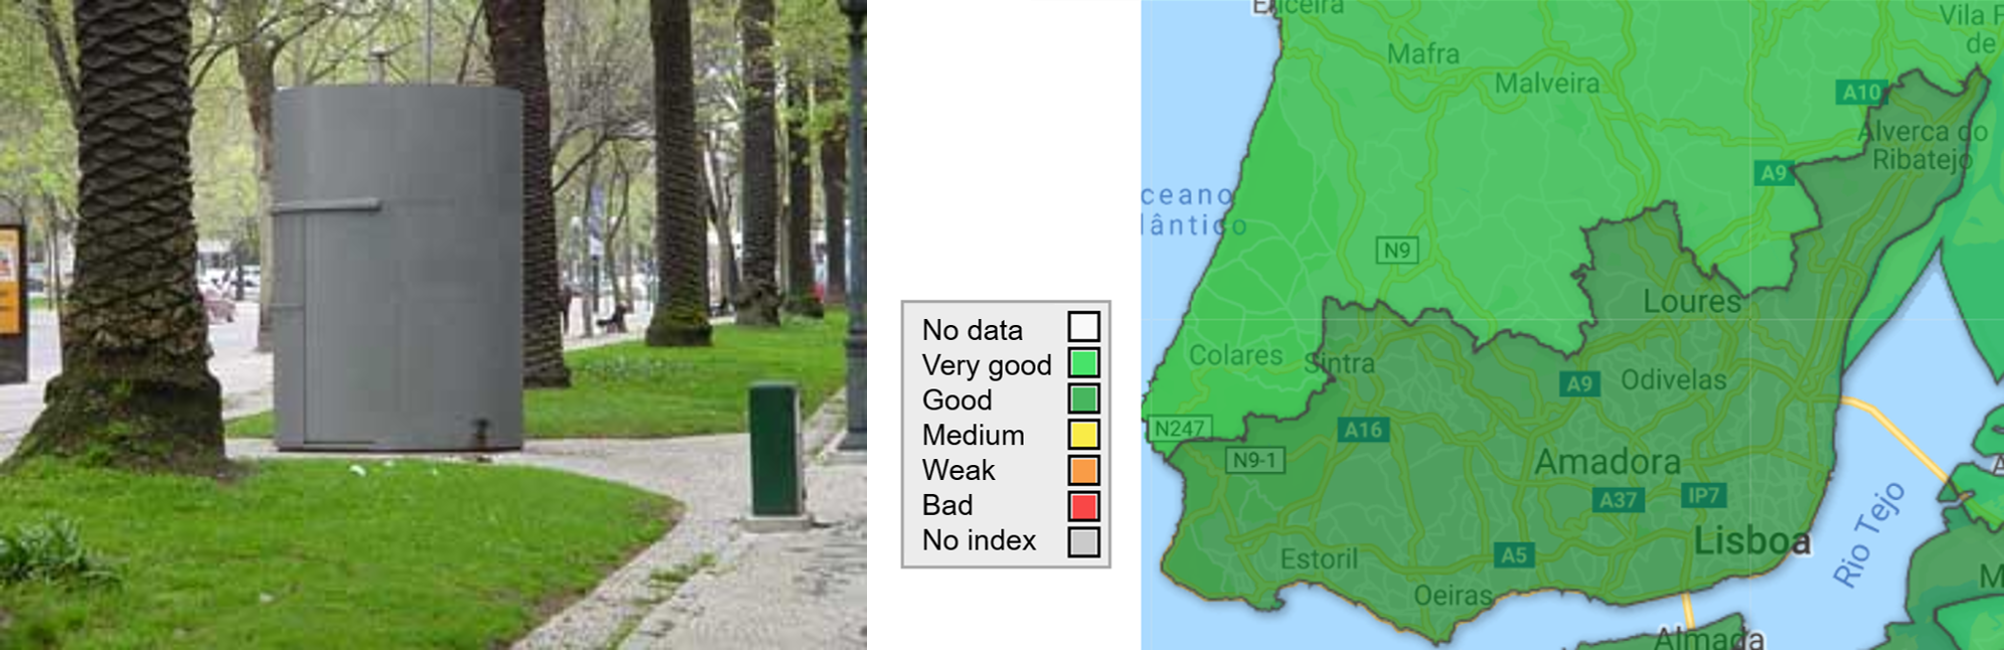
\includegraphics[width=0.9\textwidth]{./Images/ieec1.png}
\caption{Air quality monitoring and information state in Portugal.}
\label{fig:ieec1}
\end{figure}

% #############################################################################
\section{Motivation}


Throughout this and the previous decade, technology has seen big developments in the electronic and telecommunication areas, which has made possible the creation of small and low-cost sensors, compared to the ones in the aforementioned conventional systems. These sensors can be combined with electronics and technologies such as mobile communications and the \ac{IoT} to provide cheaper and more effective solutions to the current systems. With the objective of tackling the low amount of resources to model air pollution with a more granular space-time resolution, some governments are already developing initiatives with the use of these new technologies \cite{GSMA2018}.

Modelling and air quality data processing also play a big role in the control of air pollution, by providing tools for a better visualization of its evolution. This knowledge facilitates urban management, through the attainment of risk maps, which are very useful in critical situations. These provide information that raises the awareness of citizens, to change their lifestyle habits, according to the pollution in their cities, and therefore minimizing their own exposure to air pollution \cite{GSMA2018}.

In this work, from all air polluting substances, higher importance will be given to \ac{PM}, which comprises small, solid particles that are a complex mixture of chemical species, originated by a variety of sources, from anthropogenic, mainly combustion processes, to natural, such as storms, pollen and forest fires. According to \ac{EEA}, in 2017, many European cities have shown concentration values of these particles above the limit values \cite{EEA2018}. These particles can penetrate airways, lungs and blood vessels and are known to be responsible for cardiovascular and respiratory diseases as well as lung cancers. Furthermore, PM2.5 particles include pollutants such as sulfate, nitrates and black carbon, which are carcinogenic and pose the greatest risks to human health \cite{WHO2018}.

\subsection{Objectives}

The goal of this work is to develop a system for an high resolution display of PM10 concentration levels throughout the greater area of Lisbon, with the use of the latest IoT technologies available, spatial interpolation algorithms, machine learning and a web application.

The development of this system will be composed of multiple phases. First, a low-cost portable IoT PM sensing system will be developed. Second, with the help of the Lisbon air quality measures and QualAr data, several \ac{SIM}s will be assessed and compared with \ac{FBN}s in what regards spatial interpolation performance. Finally, a web application which is able to present live, fine resolution, interpolated data on PM10 concentration in the city of Lisbon will be built.

The interpolation algorithms will be evaluated based on the measures taken by the network of monitoring stations in the greater area of Lisbon and which data is available in QualAr. This database comprises validated measurement data from the year 1995 to 2017, depending on the availability of each station of the network at that time.

The development of the aforementioned system aims to tackle the current presentation of data regarding air quality, which at the moment is characterized by its coarse and poor resolution, as can be observed in \Cref{fig:ieec1}.

In \Cref{fig:methodology-flowchart} is presented a flowchart with all the steps that constitute the development of the IoT PM monitoring and presentation system.

% TODO
\begin{figure}[ht]
\centering
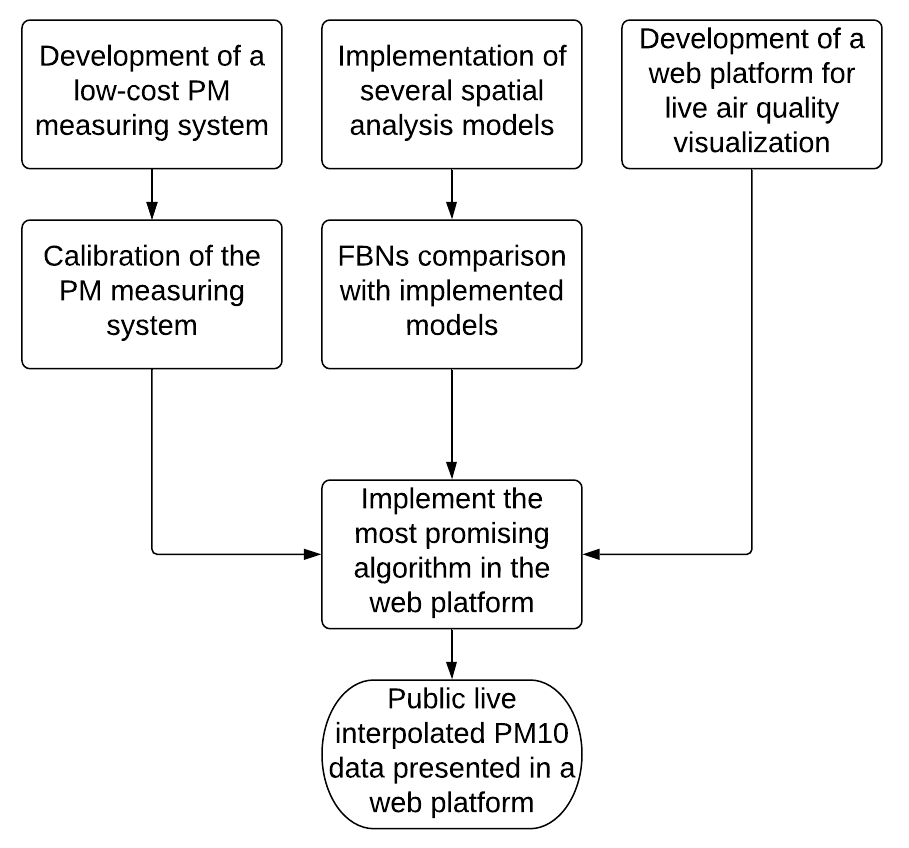
\includegraphics[width=0.64\textwidth]{./Images/methodology-flowchart.png}
\caption{Development of the IoT PM monitoring and presentation system.}
\label{fig:methodology-flowchart}
\end{figure}

% #############################################################################
\section{Claim of Contributions}

This thesis has the following contributions:

\begin{itemize}
  \item The development of an usable, affordable, and portable \ac{NB-IoT} system used for measurement of PM10 and PM2.5. In the future, this could be particularly useful for the integration of these affordable systems in the official air pollution monitoring networks.
  \item An evaluation of FBN interpolation capabilities, as well as a review of state-of-the-art SIMs, in the scope of air quality spatial interpolation applied with the state of information, in the city of Lisbon, available at the time of this thesis.
  \item The development of a web application that is able to present live interpolated PM pollution data in the city of Lisbon, with live data provided by QualAr.
  
\end{itemize}


% #############################################################################
\section{Contents}

\Cref{chap:intro} is the Introduction. It contains an overview over the topic of this work, with air pollution being revealed as a global environmental concern. A description of the motivation, objectives and contributions of this work is provided.

In \Cref{chap:back}, technologies and studies related to the field of work are reviewed, mainly in what regards performance of low-cost sensors, IoT technologies and SIMs. There is also an overview on the current forms of public presentation of available air quality data.

\Cref{chap:architecture} presents every step and methodology that will be used in this work, in detail, from the circuit development and algorithm testing, to the building of the web application prototype.

In \Cref{chap:implement}, the research and development process is concluded with an overview of the results of the built systems and the tested algorithms, along with its discussion and assessment.

In \Cref{chap:conclusion}, the main conclusions attained by this thesis are provided, along with the evaluation of its contributions and the future work that can be developed.